\section{Deep Learning}
\label{sec:deep-learning}
%Aqui introduzo o que é deep learning, dou um overview sobre o assunto (origem, definições de alguns termos mais genéricos, breve histórico)

As the method proposed in this work is a deep learning method, in this section a brief introduction on deep learning is presented, and the most commonly used terms are defined.

Deep learning is a subset of the machine learning methods that allows computer systems to improve itself with experience and data. This class of methods learns how to represent the data with a nested hierarchy of representations, with each representation defined in relation to simpler representations of the data. This procedure exploits many layers of non-linear information for feature extraction and transformation, and pattern analysis and classification~\cite{goodfellow,deepmethods}.

Most deep learning methods are defined in the context of Artificial Neural Networks~(ANN)~\cite{handsonml}. Being inspired by the biological neural network from animal brains~\cite{logicalcalculus}, ANN's are a powerful, scalable, and versatile machine learning architectures, being suitable for tackling complex problems by learning from the complex data fed to it in its training phase. An ANN with a significant number of hidden layers, that is, layers located between the input and output layers, is called Deep Artificial Neural Network~\cite{deepmethods}.  

\subsection{Convolutional Neural Networks}

Being inspired by studies over the visual cortex of the brain, Convolutional Neural Networks (CNN) are an architecture of ANN that are specialized in extracting features and information from images. Proposed back in 1998~\cite{lenet}, the basic building block of CNNs are the convolutional layers. Being based on the mathematical concept of convolution, where a function slides over another, and the integral of the pointwise multiplication is measured, the Convolutional Layer abstracts the same concept: each neuron in a convolutional layer $n$ is connected only to a receptive field in the previous layer $n-1$, not to every pixel in the image. This method allows the network to concentrate on small and localized low-level features in the first layers and then assemble these features at higher-level features on the following layers.



\subsection{Mobile-Oriented Neural Networks}

%Nesta sessão dou um overview sobre redes neurais profundas voltadas para o cenário mobile. Explico os problemas que temos no cenário mobile, como falta de memória, baixo poder de processamento, restrição energética, etc. Exemplifico com alguns trabalhos e como ajudam a contornar os problemas do mobile. Talvez introduzir a arquitetura da MobilenetV2 aqui?

Since the popularization of CNNs with AlexNet~\cite{alexnet}, the general trend has been proposing deeper models with more layers of learnable parameters, with even more complicated operations, aiming to achieve better accuracy on their tasks. However, in mobile or restrictive computing scenarios, these models with a high number of operations and computational footprint were unable to perform their tasks in an acceptable time~\cite{Howard2017CoRR}. 

Some solutions aiming to build smaller and faster CNN architectures were proposed to deal with this problem but maintaining the highly effective detection results observed by state-of-the-art methods. One of the first proposals on the scenario of NN for mobile-oriented applications was the Mobilenet~\cite{Howard2017CoRR}, in which the authors aimed at developing a CNN architecture that was competitive to the state of the art at the time but with a lightweight model, focusing first on reducing processing time but also yielding smaller models. This goal was achieved by using depthwise separable convolutions, an alternative to the classical convolutional layer that fragments it into two: the first layer is called a depthwise convolution, that filters each input channel with a single convolutional filter. The second one is called a pointwise convolution, that applies a $1 \times 1$ convolution with the objective of computing new features by a linear combination of the input channels. This layer is equivalent to a traditional convolutional layer, but with less computational operations.

Sandler et al.~\cite{Sandler2018CVPR} proposed a second version of the Mobilenet architecture, named MobilenetV2. The main contribution of this approach was the Inverted Residual with Linear Bottleneck layer. In this new module, the input is a low-dimensional compressed representation of the data, which is first expanded to a high dimension and filtered with a lightweight depthwise convolution. The results are projected back to a low-dimensional representation with a pointwise convolution. A residual connection is also inserted, connecting each low-resolution representation with the next one. This proposal improves the results of the previous version on various tasks, maintaining its low computational cost nature. The intuition is that the bottlenecks encode the model intermediate inputs and outputs, while the inner layer encapsulates the model ability to transform from lower-level concepts (such as pixels) to higher level descriptors (such as image categories). Finally, as with traditional residual connections, shortcuts enable faster training and better accuracy.

\subsection{Deep Learning for Text Detection and Recognition}
        This section describes some of the deep learning-based text detection and recognition methods.
%        \textcolor{red}{Provide the meaning of the acronyms}
        The Single Shot Text Detector (SSTD)~\cite{He2017ICCV} is a variation of the Single Shot Detector~(SSD)~\cite{Liu2016ECCV} architecture focused on text detection. This proposal outputs word-level bounding boxes, and can be divided into three parts: the convolutional module, the box prediction module and the text specific module. The convolutional and text specific modules are directly inherited from the SSD model. The text specific module can be divided into two modules: a text attention module and a hierarchical inception module. The text attention module, which comprises the convolutional layers, is responsible for learning rough spatial text features. The goal is to reduce false detections and improve the detection of ambiguous text. The hierarchical inception module has the task to aggregate multiscale features so that multiscale text can be better detected. This architecture is illustrated in Figure~\ref{fig:sstd_arch}. %\todo[inline]{Add copyright info to Appendix A}
        
        \begin{figure}[!ht]
            \centering
        	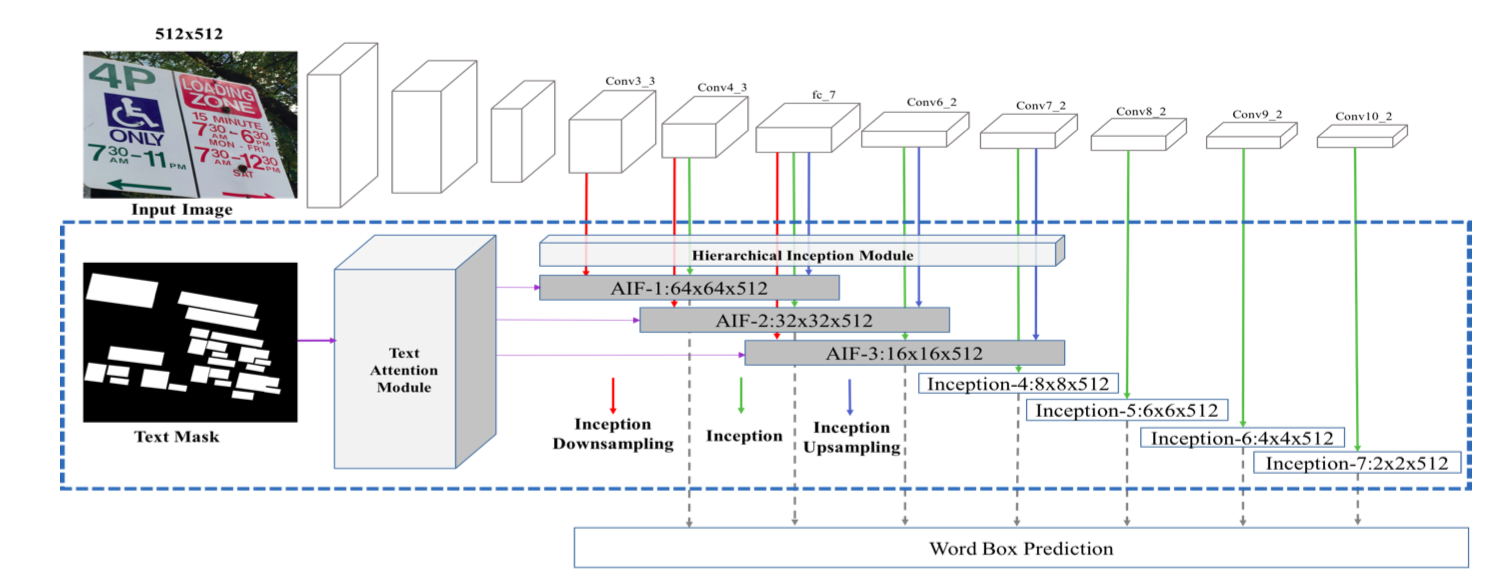
\includegraphics[width=\textwidth]{related_work/figs/SSTD_ARCH.png}
        	\caption{The SSTD architecture, figure extracted from \cite{He2017ICCV}©2017.}
        	\label{fig:sstd_arch}
        \end{figure}
        
        
        
        Liao et al.~\cite{Liao2017AAAI} proposed a fully convolutional network adapted for text detection and recognition, named TextBoxes. The authors approach inherits the VGG16~\cite{vgg} architecture, converting the last two fully-connected layers to convolutional layers by parameter downsampling. Multiple output layers are inserted after the last and some of the intermediate layers, and their outputs are aggregated, afterwards passing in a non-maximal supression process.
        
        The TextBoxes approach was later extended as the TextBoxes++~\cite{Liao2018TIP} proposal. The objective was to support the detection of arbitrary oriented bounding boxes. The proposed architecture is also a fully convolutional network. This approach extends the original proposal by predicting an arbitrary quadrilateral as a text bounding box, not only vertically oriented boxes.
        
        \begin{figure}[!ht]
            \centering
        	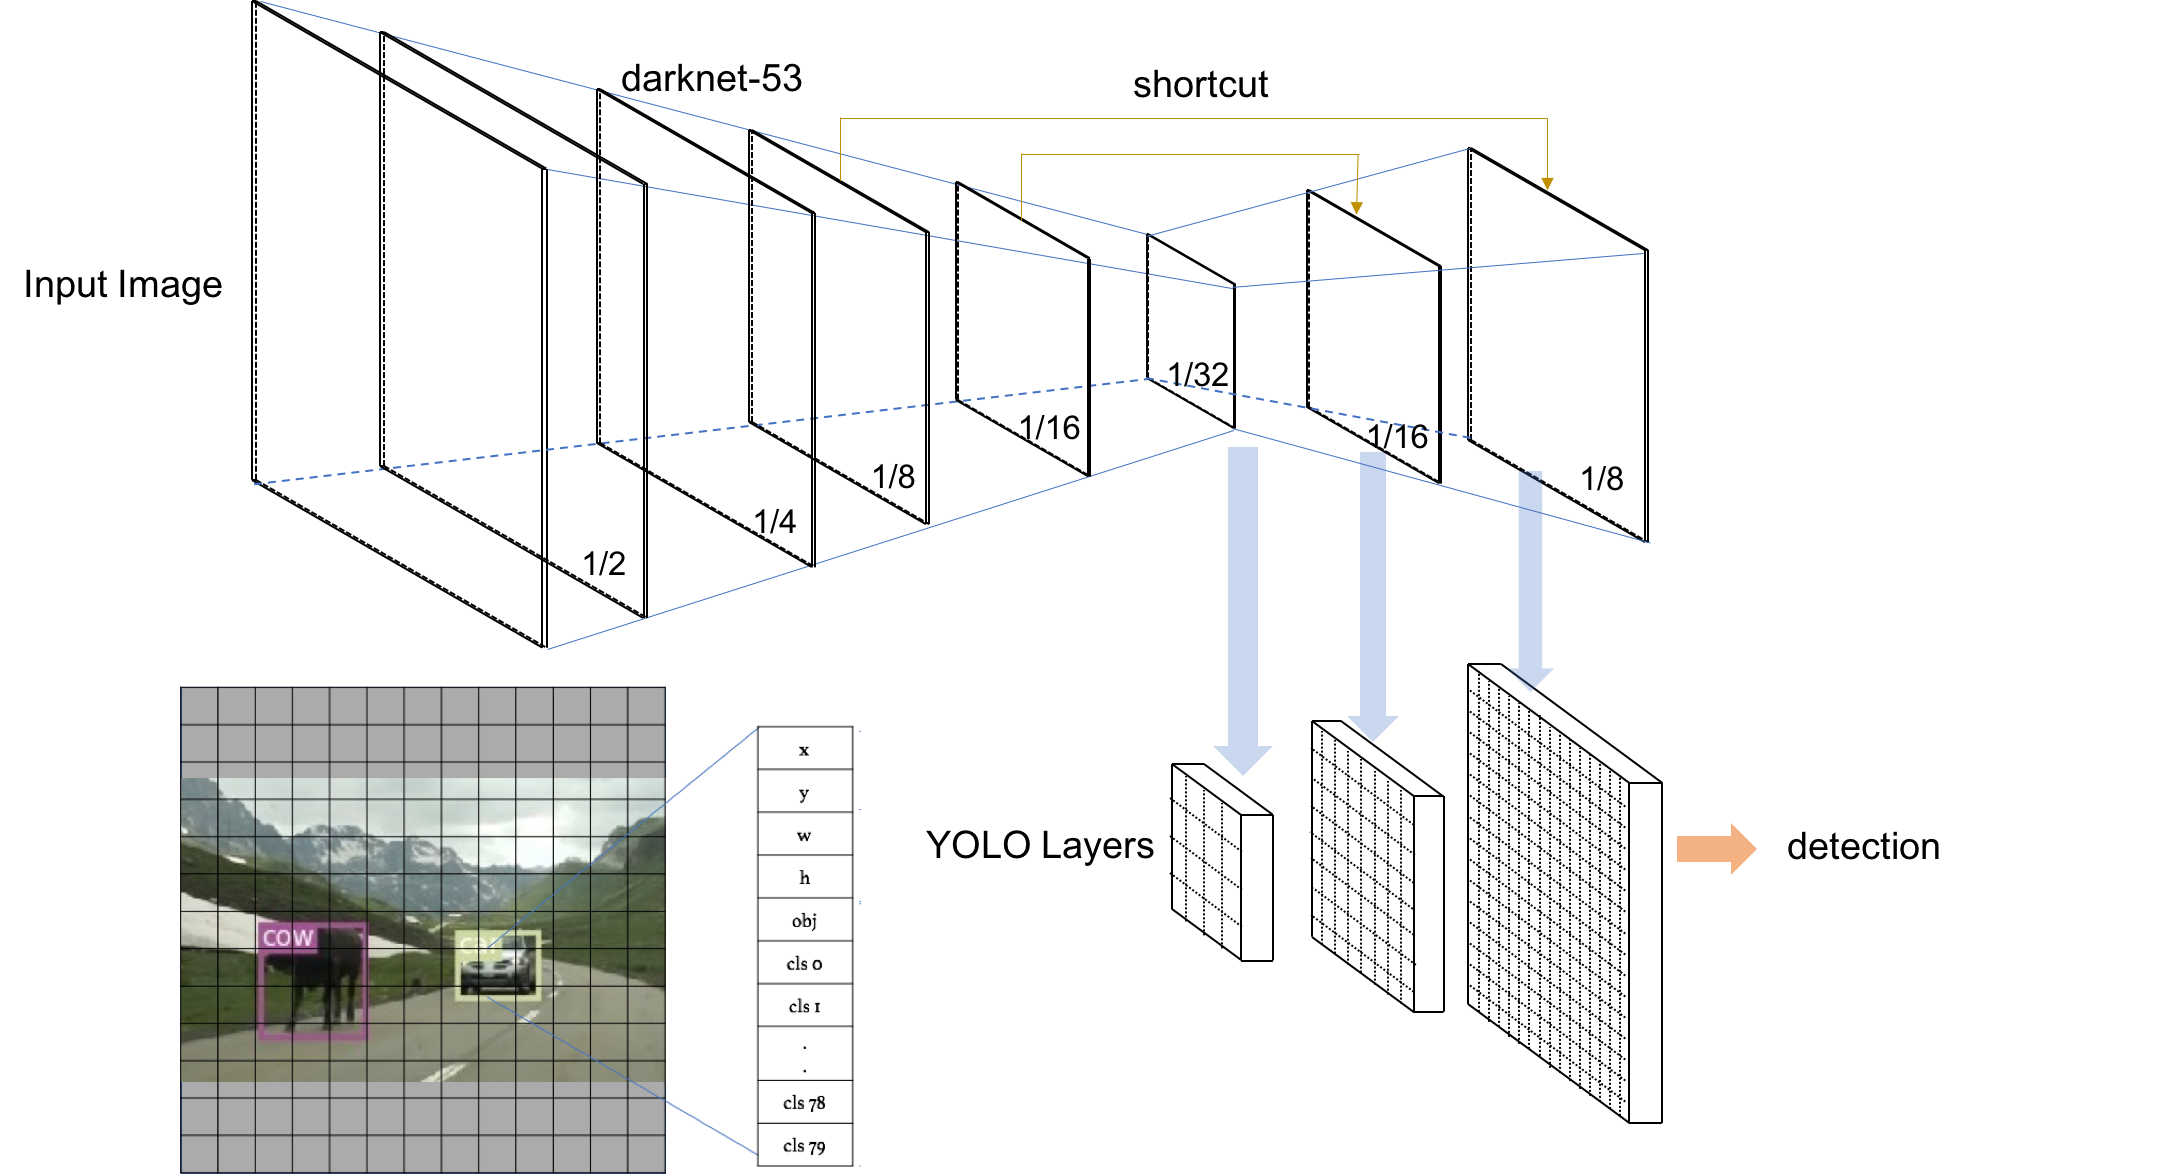
\includegraphics[width=\textwidth]{related_work/figs/YOLOV3.png}
        	\caption{Schematic of the YOLO V3 architecture ©2016.}
        	\label{fig:yolov3_arch}
        \end{figure}
        
        Another way to perform text detection on images relies on the use of methods originally proposed as object detection techniques. The YOLO V3 (You Only Look Once V3)~\cite{Redmon2018CoRR}, whose architecture can be seen in Figure~\ref{fig:yolov3_arch}, is a fully convolutional network proposed for object detection that reflects the improvements of the authors over the second version of this method. Being based on the GoogLeNet~\cite{googlenet} model, this proposal predicts bounding boxes and class probabilities directly from full images in one evaluation. The system predicts 4-coordinate bounding boxes using dimension clusters as anchor boxes and predicts an objectness score for each bounding box using logistic regression. 
        
      


